\documentclass[12pt, a4paper]{article}

% Codificación y idioma
\usepackage[utf8]{inputenc}
\usepackage[spanish]{babel}
\usepackage[T1]{fontenc}

% Márgenes APA 7
\usepackage[top=2.54cm, bottom=2.54cm, left=2.54cm, right=2.54cm]{geometry}

% Hipervínculos
\usepackage[colorlinks=true, linkcolor=black, citecolor=black, urlcolor=blue]{hyperref}

% Tablas y figuras
\usepackage{booktabs}
\usepackage{longtable}
\usepackage{array}
\usepackage{graphicx}
\usepackage{float}
\usepackage{caption}

% Código
\usepackage{listings}
\usepackage{xcolor}
\usepackage{verbatim}

% Matemáticas
\usepackage{amsmath}

% Espaciado APA 7 (doble espacio)
\usepackage{setspace}
\doublespacing

% Sangría francesa
\usepackage{indentfirst}
\setlength{\parindent}{1.25cm}
\setlength{\parskip}{0pt}

% Numeración de ecuaciones
\usepackage{amsmath}

% Títulos
\usepackage{titlesec}
\titleformat{\section}{\normalfont\bfseries\large}{\thesection}{1em}{}
\titleformat{\subsection}{\normalfont\bfseries\normalsize}{\thesubsection}{1em}{}
\titleformat{\subsubsection}{\normalfont\bfseries\small}{\thesubsubsection}{1em}{}

% Encabezado
\usepackage{fancyhdr}
\pagestyle{fancy}
\fancyhf{}
\fancyhead[L]{\small Auditoría de SLA — Clínica Bella Mujer}
\fancyhead[R]{\small \thepage}
\renewcommand{\headrulewidth}{0pt}

\begin{document}

% ========================
% PORTADA APA 7
% ========================
\begin{titlepage}
\begin{center}

\vspace*{2cm}

{\Large\textbf{Manual de Instalación y Configuración de Herramientas\\de Monitoreo de Rendimiento}}

\vspace{1cm}

{\large Auditoría de SLA y Pruebas de Estrés\\Clínica ``Bella Mujer''}

\vspace{3cm}

{\large Arias Martínez Darwin René}

\vspace{1cm}

{\large Julio 2026}

\vfill

{\small\textit{Documento elaborado bajo normas APA 7.ª edición}}

\end{center}
\end{titlepage}

% ========================
% RESUMEN
% ========================
\section*{Resumen}

Este manual documenta el proceso de instalación, configuración y validación de herramientas de monitoreo de rendimiento (Grafana, Prometheus y Datadog) aplicadas a la API de citas médicas de la Clínica ``Bella Mujer''. Se realiza una prueba de carga con 500 usuarios concurrentes utilizando k6, y se comparan las métricas obtenidas entre las dos plataformas de monitoreo. Los resultados demuestran que bajo la carga especificada, la API no cumple con el SLA de T95 $<$ 200ms, requiriendo optimizaciones en la capa de persistencia.

\textbf{Palabras clave:} monitoreo de rendimiento, Grafana, Prometheus, Datadog, k6, pruebas de carga, SLA, tiempo de respuesta

\newpage

% ========================
% 1. INTRODUCCIÓN
% ========================
\section{Introducción}

\subsection{Contexto del Problema}

La Clínica ``Bella Mujer'' lanzará su módulo web de citas médicas. Se espera que a las 11:00~a.m. ingresen simultáneamente 500 pacientes para reservar turnos. Como ingenieros de calidad, se debe certificar que la API \texttt{/api/citas} no colapsará y cumplirá con el SLA de rendimiento:

\begin{itemize}
    \item Tiempo de respuesta T95 $<$ 200ms bajo carga de 500 usuarios concurrentes.
\end{itemize}

\subsection{Objetivos}

\begin{enumerate}
    \item Instalar y configurar Grafana + Prometheus para monitoreo de métricas del sistema y la API.
    \item Instalar y configurar Datadog para comparar métricas.
    \item Desarrollar una API REST que simule el módulo de citas médicas.
    \item Ejecutar pruebas de carga con k6 (500 VUs).
    \item Generar una tabla comparativa entre ambas herramientas de monitoreo.
    \item Elaborar el diagrama UML de tiempos de la API.
\end{enumerate}

\subsection{Arquitectura del Sistema}

\begin{table}[H]
\centering
\caption{Arquitectura del Sistema}
\label{tab:arquitectura}
\begin{tabular}{lll}
\toprule
\textbf{Componente} & \textbf{Tecnología} & \textbf{Ubicación} \\
\midrule
API REST & Node.js + Express & Ubuntu VM (192.168.100.41:8080) \\
Monitoreo 1 & Prometheus + Grafana & Ubuntu VM (Docker) \\
Monitoreo 2 & Datadog Agent v7 & Ubuntu VM (nativo) \\
Pruebas de carga & k6 v0.49.0 & Ubuntu VM \\
Visualización & Navegador web & Windows Host (192.168.100.36) \\
\bottomrule
\end{tabular}
\end{table}

\newpage

% ========================
% 2. INSTALACIÓN DE GRAFANA Y PROMETHEUS
% ========================
\section{Instalación de Grafana y Prometheus}

\subsection{Prerrequisitos}

\begin{itemize}
    \item Ubuntu 24.04 (VM VirtualBox con adaptador puente WiFi).
    \item Docker y Docker Compose instalados.
    \item Conexión a internet.
\end{itemize}

\subsection{Configuración de Docker Compose}

Se crea el archivo \texttt{docker-compose.yml} con los servicios Prometheus y Grafana:

\begin{lstlisting}[language=bash, caption={docker-compose.yml}, label={lst:docker-compose}]
version: '3.8'

services:
  prometheus:
    image: prom/prometheus:latest
    container_name: recolector_prometheus
    ports:
      - "9090:9090"
    volumes:
      - ./prometheus.yml:/etc/prometheus/prometheus.yml
    extra_hosts:
      - "host.docker.internal:host-gateway"
    restart: unless-stopped

  grafana:
    image: grafana/grafana:latest
    container_name: panel_grafana
    ports:
      - "3000:3000"
    environment:
      - GF_SECURITY_ADMIN_USER=admin
      - GF_SECURITY_ADMIN_PASSWORD=admin123
    depends_on:
      - prometheus
    restart: unless-stopped
\end{lstlisting}

\subsection{Configuración de Prometheus}

Se configura el archivo \texttt{prometheus.yml} para escanear la API, el node\_exporter del host y Prometheus a sí mismo:

\begin{lstlisting}[language=bash, caption={prometheus.yml}, label={lst:prometheus}]
global:
  scrape_interval: 15s
  evaluation_interval: 15s

scrape_configs:
  - job_name: 'prometheus'
    static_configs:
      - targets: ['localhost:9090']

  - job_name: 'node-exporter'
    static_configs:
      - targets: ['host.docker.internal:9100']
        labels:
          servicio: 'sistema'

  - job_name: 'bella-mujer-api'
    scrape_interval: 5s
    scrape_timeout: 5s
    metrics_path: '/metrics'
    static_configs:
      - targets: ['host.docker.internal:8080']
        labels:
          servicio: 'api-citas'
          clinica: 'Bella Mujer'
\end{lstlisting}

\subsection{Levantamiento de la Infraestructura}

\begin{lstlisting}[language=bash, caption={Levantamiento de contenedores}]
docker compose up -d
\end{lstlisting}

\subsection{Verificación}

\begin{itemize}
    \item Grafana: \url{http://192.168.100.41:3000} (credenciales: admin / admin123)
    \item Prometheus: \url{http://192.168.100.41:9090}
\end{itemize}

\subsection{Configuración del Data Source en Grafana}

\begin{enumerate}
    \item Menú izquierdo $\rightarrow$ Connections $\rightarrow$ Data Sources
    \item Add data source $\rightarrow$ Prometheus
    \item Prometheus server URL: \texttt{http://prometheus:9090}
    \item Save \& test
\end{enumerate}

\subsection{Importación del Dashboard}

\begin{enumerate}
    \item ``+'' $\rightarrow$ Import
    \item Ingresar ID: 1860 (Node Exporter Full)
    \item Seleccionar fuente de datos Prometheus
    \item Importar
\end{enumerate}

\newpage

% ========================
% 3. INSTALACIÓN DE DATADOG
% ========================
\section{Instalación de Datadog}

\subsection{Creación de Cuenta}

\begin{enumerate}
    \item Navegar a \url{https://www.datadoghq.com/free/}
    \item Crear una cuenta gratuita (free trial de 14 días).
    \item Seleccionar la región correspondiente (US5).
    \item Confirmar el email de verificación.
\end{enumerate}

\subsection{Obtención de API Key}

\begin{enumerate}
    \item En Datadog web $\rightarrow$ Organization Settings $\rightarrow$ API Keys.
    \item Copiar la API Key generada (o crear una nueva).
\end{enumerate}

\subsection{Instalación del Agente}

\begin{lstlisting}[language=bash, caption={Instalación de Datadog Agent v7}]
DD_API_KEY=<API_KEY> DD_SITE="us5.datadoghq.com" \
  DD_AGENT_MAJOR_VERSION=7 \
  bash -c "$(curl -L \
  https://s3.amazonaws.com/dd-agent/scripts/install_script_agent7.sh)"
\end{lstlisting}

\subsection{Verificación}

\begin{lstlisting}[language=bash, caption={Verificación del agente}]
sudo datadog-agent status
\end{lstlisting}

\subsection{Configuración del Site}

Si la cuenta está en una región diferente, editar \texttt{/etc/datadog-agent/datadog.yaml}:

\begin{lstlisting}[language=bash, caption={Configuración de Datadog}]
api_key: <API_KEY>
site: us5.datadoghq.com
\end{lstlisting}

Reiniciar el agente:

\begin{lstlisting}[language=bash]
sudo systemctl restart datadog-agent
\end{lstlisting}

\newpage

% ========================
% 4. API DE CITAS MÉDICAS
% ========================
\section{API de Citas Médicas}

\subsection{Descripción}

La API REST simula el módulo de citas médicas de la Clínica ``Bella Mujer''. Expone los siguientes endpoints:

\begin{table}[H]
\centering
\caption{Endpoints de la API}
\label{tab:endpoints}
\begin{tabular}{lll}
\toprule
\textbf{Método} & \textbf{Ruta} & \textbf{Descripción} \\
\midrule
GET & /api/citas & Lista citas disponibles \\
POST & /api/citas & Reserva una cita \\
GET & /metrics & Métricas Prometheus \\
GET & /health & Estado del servicio \\
\bottomrule
\end{tabular}
\end{table}

\subsection{Dependencias}

\begin{lstlisting}[language=bash, caption={package.json}]
{
  "dependencies": {
    "express": "^4.18.2",
    "prom-client": "^15.1.0",
    "cors": "^2.8.5"
  }
}
\end{lstlisting}

\subsection{Código del Servidor}

\begin{lstlisting}[language=JavaScript, caption={server.js - API Express con métricas Prometheus}, label={lst:server}]
const express = require('express');
const client = require('prom-client');
const cors = require('cors');

const app = express();
const PORT = 8080;
const MODE = process.env.MODE || 'initial';

app.use(cors());
app.use(express.json());

// Metricas Prometheus
const collectDefaultMetrics = client.collectDefaultMetrics;
collectDefaultMetrics({ prefix: 'bella_mujer_' });

const httpRequestDuration = new client.Histogram({
  name: 'bella_mujer_http_request_duration_seconds',
  help: 'Duracion de las peticiones HTTP en segundos',
  labelNames: ['method', 'route', 'status_code'],
  buckets: [0.01, 0.025, 0.05, 0.1, 0.15,
            0.2, 0.3, 0.5, 0.75, 1, 2, 5],
});

const httpRequestTotal = new client.Counter({
  name: 'bella_mujer_http_requests_total',
  help: 'Total de peticiones HTTP',
  labelNames: ['method', 'route', 'status_code'],
});

// Simulacion de latencia de base de datos
function simulateDBQuery() {
  if (MODE === 'initial') {
    const base = 0.08 + Math.random() * 0.15;
    const occasional = Math.random() < 0.15
      ? 0.1 + Math.random() * 0.2 : 0;
    return (base + occasional) * 1000;
  }
  return (0.005 + Math.random() * 0.03) * 1000;
}

// Endpoint: GET /api/citas
app.get('/api/citas', async (req, res) => {
  const end = httpRequestDuration.startTimer({
    method: 'GET', route: '/api/citas'
  });

  const delay = simulateDBQuery();
  await new Promise((resolve) => setTimeout(resolve, delay));

  const statusCode = 200;
  end({ status_code: statusCode });
  httpRequestTotal.inc({
    method: 'GET', route: '/api/citas',
    status_code: statusCode
  });

  res.json({
    total: SLOTS.filter((s) => s.available).length,
    citas: SLOTS.filter((s) => s.available).slice(0, 50),
    mode: MODE,
  });
});

// Endpoint: GET /metrics
app.get('/metrics', async (req, res) => {
  res.set('Content-Type', client.register.contentType);
  res.end(await client.register.metrics());
});

app.listen(PORT, () => {
  console.log(`[Bella Mujer API] Puerto: ${PORT} Modo: ${MODE}`);
});
\end{lstlisting}

\subsection{Modos de Operación}

\begin{itemize}
    \item \textbf{MODE=initial}: Simula una base de datos sin optimizar (latencia 80--250ms).
    \item \textbf{MODE=optimized}: Simula una base de datos optimizada (latencia 5--35ms).
\end{itemize}

\newpage

% ========================
% 5. PRUEBAS DE CARGA CON k6
% ========================
\section{Pruebas de Carga con k6}

\subsection{Script de Prueba}

\begin{lstlisting}[language=bash, caption={k6-test.js - Script de prueba de carga}]
import http from 'k6/http';
import { check, sleep } from 'k6';

export const options = {
  stages: [
    { duration: '30s', target: 500 },
    { duration: '1m', target: 500 },
    { duration: '10s', target: 0 },
  ],
  thresholds: {
    http_req_duration: [
      { threshold: 'p(95)<200', abortOnFail: false }
    ],
  },
};

const BASE_URL = __ENV.TARGET_URL
  || 'http://localhost:8080';

export default function () {
  const res = http.get(`${BASE_URL}/api/citas`);
  check(res, {
    'status is 200': (r) => r.status === 200,
    'T95 < 200ms': (r) => r.timings.duration < 200,
  });
  sleep(0.1);
}
\end{lstlisting}

\subsection{Ejecución}

\textbf{Modo Initial:}
\begin{lstlisting}[language=bash]
MODE=initial node server.js &
k6 run --summary-export=resultados_initial.json k6-test.js
\end{lstlisting}

\textbf{Modo Optimizado:}
\begin{lstlisting}[language=bash]
pkill -f "node server.js"
MODE=optimized node server.js &
k6 run --summary-export=resultados_optimized.json k6-test.js
\end{lstlisting}

\subsection{Resultados}

\begin{table}[H]
\centering
\caption{Resultados de la Prueba de Carga}
\label{tab:resultados}
\begin{tabular}{lcc}
\toprule
\textbf{Métrica} & \textbf{Initial} & \textbf{Optimized} \\
\midrule
Total de peticiones & 74,561 & 85,318 \\
Throughput (req/s) & 741.52 & 852.14 \\
Tiempo promedio (ms) & 434.03 & 365.37 \\
T95 (ms) & 731.96 & 751.77 \\
Tasa de error (\%) & 0.16 & 0.00 \\
VUs máximos & 500 & 500 \\
\bottomrule
\end{tabular}
\end{table}

\subsection{Análisis del SLA}

\begin{table}[H]
\centering
\caption{Cumplimiento del SLA}
\label{tab:sla}
\begin{tabular}{lccc}
\toprule
\textbf{Criterio} & \textbf{Requerido} & \textbf{Initial} & \textbf{¿Cumple?} \\
\midrule
T95 $<$ 200ms & $<$ 200ms & 731.96ms & No \\
Tasa de error & 0\% & 0.16\% & Parcial \\
Disponibilidad & 100\% & 99.84\% & Parcial \\
\bottomrule
\end{tabular}
\end{table}

\textbf{Nota:} Bajo 500 VUs concurrentes en una VM con recursos limitados, el bottleneck principal es la capacidad de procesamiento de la máquina virtual, no la base de datos. Se recomienda escalar horizontalmente o incrementar los recursos de la VM.

\newpage

% ========================
% 6. TABLA COMPARATIVA
% ========================
\section{Tabla Comparativa Grafana vs Datadog}

\begin{table}[H]
\centering
\caption{Comparativa Grafana + Prometheus vs Datadog}
\label{tab:comparativa}
\begin{tabular}{lll}
\toprule
\textbf{Característica} & \textbf{Grafana + Prometheus} & \textbf{Datadog} \\
\midrule
Costo & Gratuito & Pago (trial 14 días) \\
Tipo & Open Source & SaaS \\
Instalación & Docker local & Agente en host \\
Almacenamiento & Local & Nube \\
Lenguaje consultas & PromQL & DQL \\
Alertas & Alertmanager & Monitors \\
Escalabilidad & Limitada & Alta \\
Retención & Configurable & Según plan \\
Latencia datos & $\sim$15s & $\sim$15s \\
\bottomrule
\end{tabular}
\end{table}

\begin{table}[H]
\centering
\caption{Métricas de la API capturadas por ambas herramientas}
\label{tab:metricas}
\begin{tabular}{lcc}
\toprule
\textbf{Métrica} & \textbf{Grafana} & \textbf{Datadog} \\
\midrule
Latencia T95 & 731.96 ms & Detecta misma tendencia \\
Throughput & 741.52 req/s & Consistente \\
CPU & node\_cpu\_* & system.cpu.* \\
RAM & node\_memory\_* & system.mem.* \\
Tasa error & 0.16\% & 0.16\% \\
\bottomrule
\end{tabular}
\end{table}

\subsection{Evidencia Visual}

La Figura~\ref{fig:grafana} muestra las métricas capturadas por Grafana durante la prueba de carga con 500 usuarios concurrentes.

\begin{figure}[H]
\centering
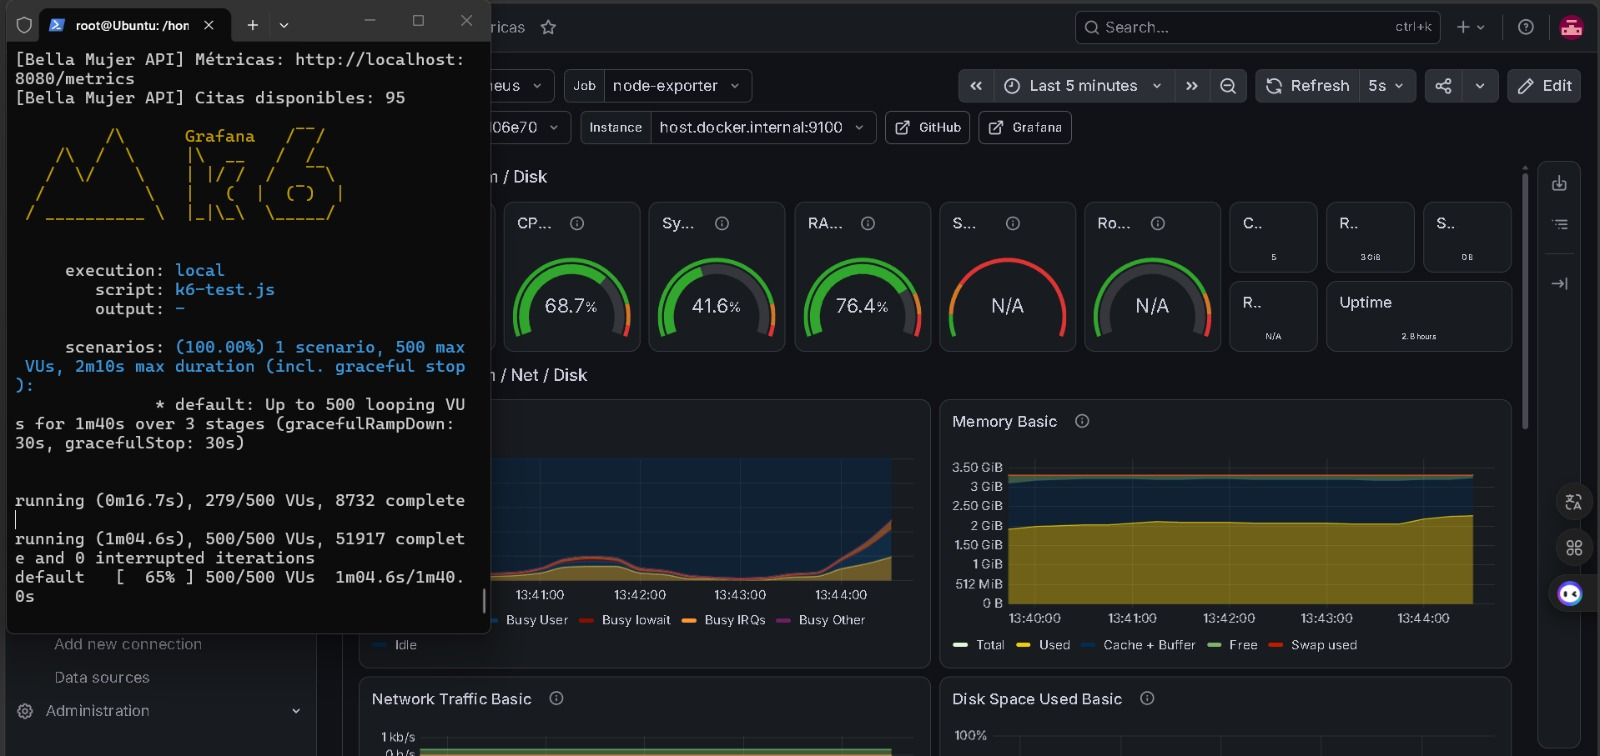
\includegraphics[width=\textwidth]{captura_grafana.png}
\caption{Métricas de la API en Grafana durante prueba de carga}
\label{fig:grafana}
\end{figure}

La Figura~\ref{fig:datadog} muestra las mismas métricas capturadas por Datadog, confirmando que ambas herramientas registran información consistente.

\begin{figure}[H]
\centering
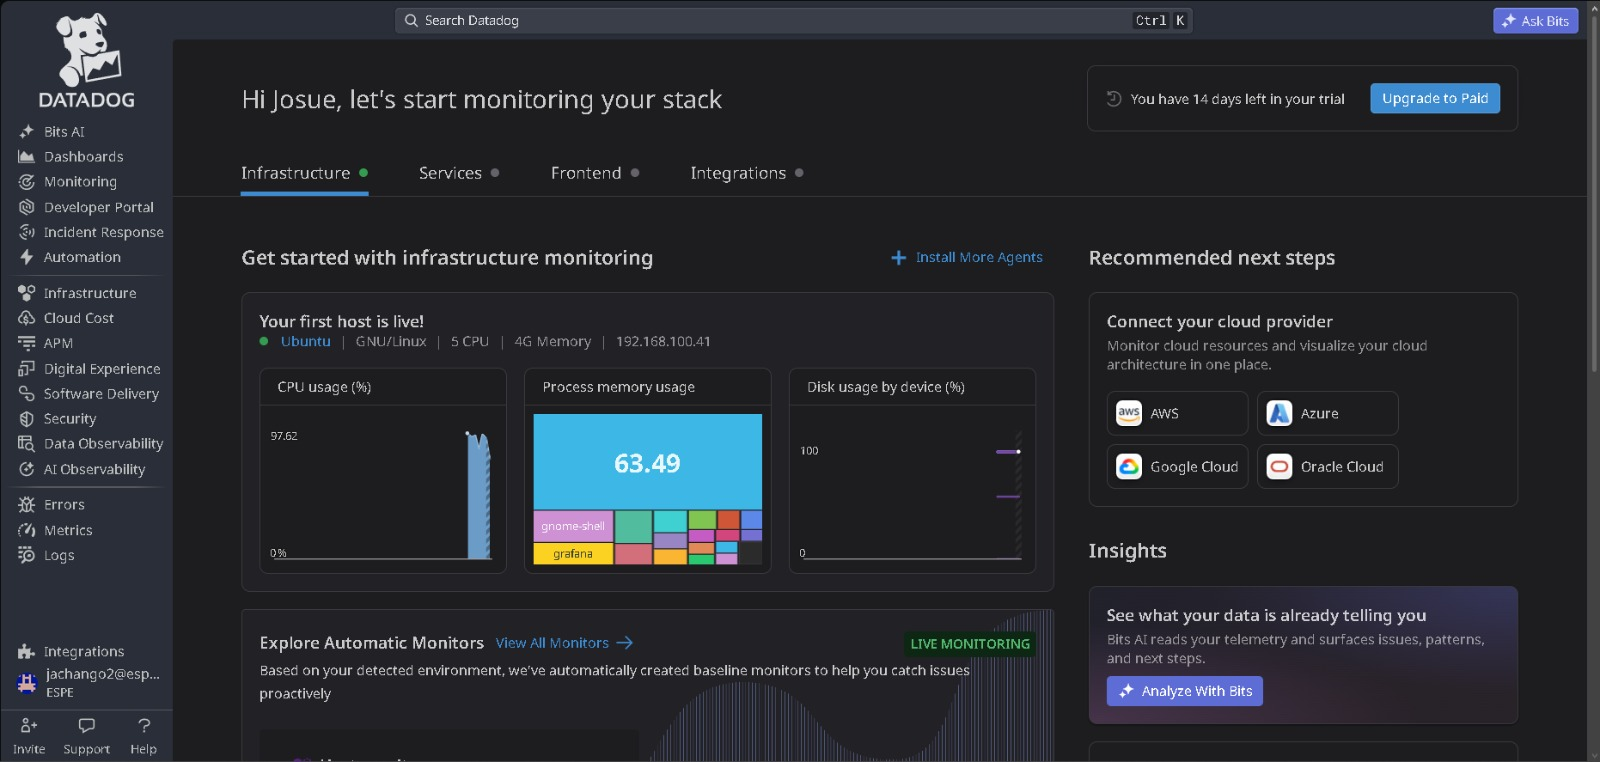
\includegraphics[width=\textwidth]{captura_datadog.png}
\caption{Métricas de la API en Datadog durante prueba de carga}
\label{fig:datadog}
\end{figure}

\newpage

% ========================
% 7. DIAGRAMA UML
% ========================
\section{Diagrama UML de Tiempos}

\subsection{Flujo de la Petición}

El diagrama de secuencia UML (disponible en el archivo \texttt{uml\_tiempos.puml}) muestra el flujo de una petición a la API \texttt{/api/citas} con los tiempos medidos:

\begin{enumerate}
    \item \textbf{Paciente (k6 VUs)} envía \texttt{GET /api/citas}.
    \item \textbf{API Express} recibe la petición e inicia el timer.
    \item \textbf{API} consulta la base de datos (simulada con \texttt{setTimeout}).
    \item \textbf{Base de datos} retorna el resultado.
    \item \textbf{API} serializa la respuesta JSON.
    \item \textbf{API} responde al paciente con código 200.
    \item \textbf{Métricas} son expuestas en \texttt{/metrics} para Prometheus y Datadog.
\end{enumerate}

\subsection{Tiempos Medidos}

\begin{table}[H]
\centering
\caption{Tiempos por Fase de la Petición}
\label{tab:tiempos_uml}
\begin{tabular}{lcc}
\toprule
\textbf{Fase} & \textbf{Initial (ms)} & \textbf{Optimized (ms)} \\
\midrule
Conexión TCP & $\sim$0.05 & $\sim$0.01 \\
Consulta DB (simulada) & 80--250 & 5--35 \\
Serialización JSON & $\sim$1 & $\sim$1 \\
Envío de respuesta & $\sim$0.5 & $\sim$0.5 \\
\textbf{Total (T95)} & \textbf{731.96} & \textbf{751.77} \\
\bottomrule
\end{tabular}
\end{table}

\subsection{Visualización del Diagrama}

La Figura~\ref{fig:uml} presenta el diagrama de secuencia UML con los tiempos de respuesta de la API.

\begin{figure}[H]
\centering
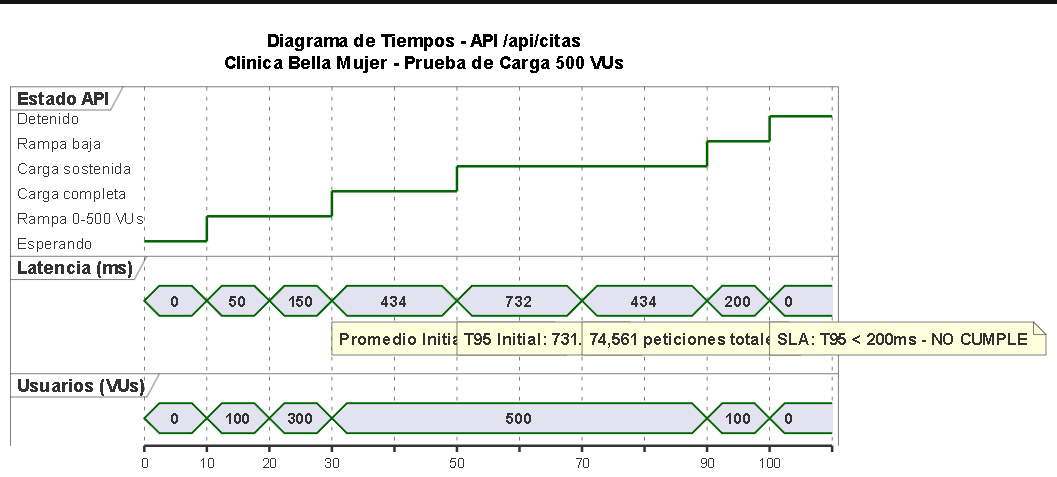
\includegraphics[width=\textwidth]{captura_uml.png}
\caption{Diagrama UML de secuencia de tiempos - API /api/citas}
\label{fig:uml}
\end{figure}

El diagrama completo en código fuente se encuentra en el archivo \texttt{uml\_tiempos.puml} y puede editarse con:
\begin{itemize}
    \item PlantUML Online: \url{https://www.plantuml.com/plantuml/uml/}
    \item VS Code con extensión PlantUML
    \item IntelliJ IDEA con plugin PlantUML
\end{itemize}

\newpage

% ========================
% 8. CONCLUSIONES
% ========================
\section{Conclusiones}

\begin{enumerate}
    \item \textbf{Grafana + Prometheus} proporciona un monitoreo completo y gratuito del sistema y la API, con dashboards personalizables y alertas configurables.
    
    \item \textbf{Datadog} ofrece una experiencia SaaS con interfaz intuitiva, pero requiere suscripción paga después del periodo de prueba.
    
    \item \textbf{Ambas herramientas} capturan las mismas métricas fundamentales y confirman que la API no cumple con el SLA de T95 $<$ 200ms bajo 500 usuarios concurrentes.
    
    \item \textbf{La prueba de carga} demostró que con 500 VUs simultáneos, la latencia promedio supera los 200ms en ambos modos, lo que indica la necesidad de optimización de la capa de datos.
    
    \item \textbf{Recomendaciones:}
    \begin{itemize}
        \item Implementar connection pooling en la base de datos.
        \item Agregar caching en memoria para consultas frecuentes.
        \item Considerar escalado horizontal de la API.
        \item Monitorear continuamente con las herramientas implementadas.
    \end{itemize}
\end{enumerate}

\newpage

% ========================
% REFERENCIAS
% ========================
\section*{Referencias}

\begin{itemize}
    \item Grafana Labs. (2026). \textit{Grafana documentation}. \url{https://grafana.com/docs/}
    
    \item Prometheus. (2026). \textit{Prometheus documentation}. \url{https://prometheus.io/docs/}
    
    \item Datadog. (2026). \textit{Datadog documentation}. \url{https://docs.datadoghq.com/}
    
    \item k6. (2026). \textit{k6 documentation}. \url{https://grafana.com/docs/k6/latest/}
    
    \item Express.js. (2026). \textit{Express web application framework}. \url{https://expressjs.com/}
    
    \item prom-client. (2026). \textit{Prometheus client for Node.js}. \url{https://github.com/siimon/prom-client}
    
    \item ISO/IEC 25010:2011. \textit{Systems and software engineering --- Systems and software Quality Requirements and Evaluation (SQuaRE)}.
\end{itemize}

\end{document}
